\chapter{Practical details}

\section{Length of recording}
\begin{figure}[H]
\begin{subfigure}[b]{0.96\textwidth}
    \centering
    \includegraphics[width=0.7\textwidth]{Figures/ChalkCloseFull1Sec.png}
\end{subfigure}
\vskip \baselineskip
\begin{subfigure}[b]{0.96\textwidth}
    \centering
    \includegraphics[width=0.7\textwidth]{Figures/ChalkCloseFull10Sec.png}
\end{subfigure}
\vskip \baselineskip
\begin{subfigure}[b]{0.96\textwidth}
    \centering
    \includegraphics[width=0.7\textwidth]{Figures/ChalkCloseFull120Sec.png}
\end{subfigure}
\caption{Figures depict from SRP-PHAT localization results, for recording length 1sec (top), 10sec (middle) and 120sec (bottom). Relative dB are plotted here}
\label{fig:4mic1srcRedun}
\end{figure}


\section{Filter Design}
\label{app:filterdesign}

The low pass and high pass filter are design using Matlab Filter Designer. Design specification of the low pass is $fs = 131072 Hz$, minimum order, FIR equiripple, stop band $80dB$, stop band frequency $300Hz$ and pass band frequency $100Hz$. The filter order is 1659. Figure \ref{fig:filterlowpass300} and \ref{fig:filterhighpass300} shows the frequency and impulse response of each filters.

\begin{figure}[H]
    \centering
\vskip \baselineskip
\begin{subfigure}[b]{0.96\textwidth}
    \centering
    \includegraphics[width=0.7\textwidth]{Figures/lowpass300zommed.png}
\end{subfigure}
\vskip \baselineskip
\begin{subfigure}[b]{0.96\textwidth}
    \centering
    \includegraphics[width=0.7\textwidth]{Figures/lowpass300IR.png}
\end{subfigure}
\caption{Figures depict the frequency response and impulse response of the 300Hz low pass filter}
\label{fig:filterlowpass300}
\end{figure}

Design specification of the High pass is $fs = 131072 Hz$, minimum order, FIR equiripple, stop band $80dB$, stop band frequency $100Hz$ and pass band frequency $300Hz$. The filter order is 1801.
\begin{figure}[H]
    \centering
\vskip \baselineskip
\begin{subfigure}[b]{0.96\textwidth}
    \centering
    \includegraphics[width=0.7\textwidth]{Figures/highpass300zoomed.png}
\end{subfigure}
\vskip \baselineskip
\begin{subfigure}[b]{0.96\textwidth}
    \centering
    \includegraphics[width=0.7\textwidth]{Figures/highpass300IR.png}
\end{subfigure}
\caption{Figures depict the frequency response and impulse response of the 300Hz High pass filter}
\label{fig:filterhighpass300}
\end{figure}

In order to zero-phase filter the signal, the signal are filter once, then inverted and filer again. Matlab function filtfilt is used.

\section{Cross-correlation levels against recording length}
\begin{figure}[!ht]
    \centering
    \includegraphics[width=0.8\textwidth]{Figures/20200500.png}
    \caption{Magnitude of the cross-correlation of a pair of microphones. No additive noise. The blue line is the magnitude of the cross correlation with PHAT weighting for a 50Hz sin wave with different recording time 500s (blue), 200s (orange) and 20s (orange)}
    \label{fig:xcorr20500hz}
\end{figure}


\section{Generation of white noise}

\section{Generation of pink noise}

\section{Simulating a tetrahedral array}

\section{Other system diagram}
\begin{figure}[H]
    \centering
    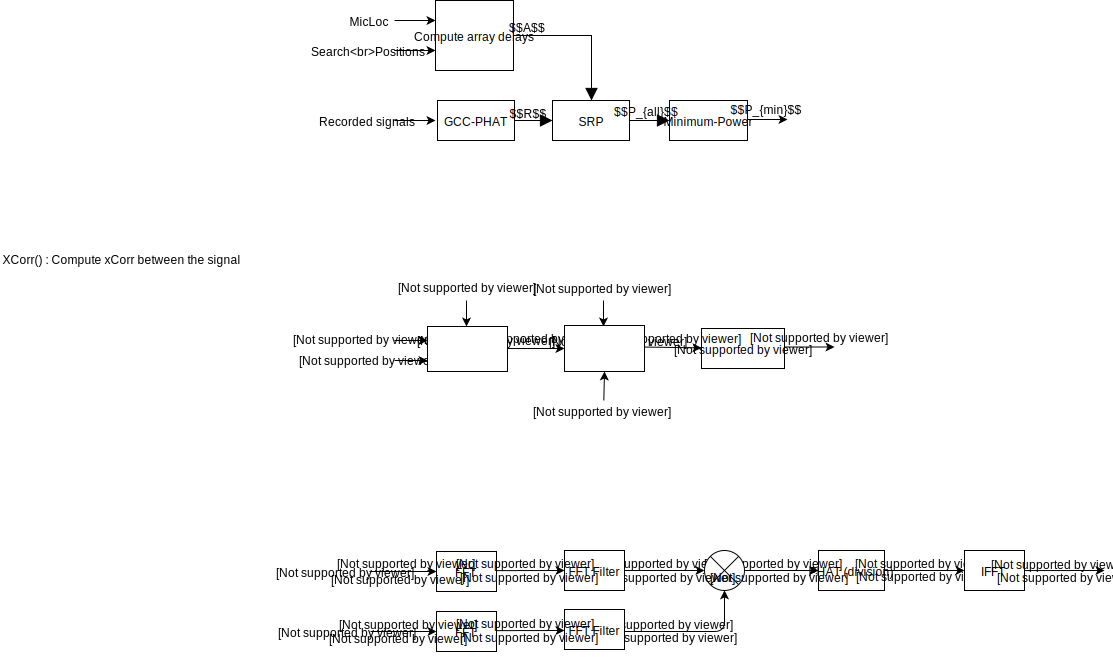
\includegraphics[width=1\textwidth]{Figures/system2.png}
    \caption{SRP block + Minimum Power}
    \label{fig:system2}
\end{figure}

\section{Microphone sensitivity}
The sensitivities of the microphones used for the tetrahedral array are tabulated below.
\begin{table}
    \begin{tabular}{ll} \toprule
	{Mic}	&	{Sensitivity}\\
	    \bottomrule 
	    M_1   &   6.694 mV/Pa                   \\
	    M_2   &   5.743 mV/Pa                        \\
	    M_3   &                                 \\
		M_4   &                                 \\
		\bottomrule 
	\end{tabular}
\end{table}